\documentclass[tikz,border=2cm,dvipsnames,rgb]{standalone}

\usepackage{amsmath,amssymb,amsfonts}
\usetikzlibrary{calc,
fit,
shapes.misc,
shapes.geometric,
arrows.meta,
fadings,
matrix,
chains,
scopes,
positioning}

\usepackage{pgfplots}
\usepackage{pgfplotstable}
\pgfplotsset{compat=1.18}



\usepackage[]{fontspec}

\setmainfont{Latin Modern Roman}
\setmonofont{Latin Modern Math}
\renewcommand{\textsc}[1]{{\fontfamily{lmr}\selectfont \scshape #1}}

\usepackage[]{bm}

\makeatletter
\@ifundefined{fromRoot}{\newcommand{\fromRoot}[1]{../../#1}}{}

\def\input@path{{../..}{..}{.}{./svg}{./pgfplots}{./tikzpicture}}
%or: \def\input@path{{/path/to/folder/}{/path/to/other/folder/}}
\makeatother

\newcommand*{\gf}[1]{\acrshort{gf}($#1$)}%
\newcommand*{\mpn}[1]{\bm{P}_{#1}}%
\newcommand*{\pn}[1]{%
  \ifthenelse{\equal{#1}{}}{$\mpn{0}$}{$\mpn{#1}$}%
}%

\newcommand*{\pk}[3]{%
  \ifthenelse{\equal{#1}{#2}}{\textcolor{red}{\phantom{.}$p_0$\phantom{.}}}{\phantom{.}$p_#3$\phantom{.}}%
}%


\newcommand*{\placeholder}{
\includegraphics[width=\linewidth, height=.25\textheight, keepaspectratio = true]{figures/certified_xilinx.png}}%

\newcommand*{\snr}{\acrshort{snr}}%
\newcommand*{\snrs}{\acrshortpl{snr}}%

\newcommand*{\mpd}[0]{p_\Delta}%
\newcommand*{\mpo}[0]{p_\omega}%
\newcommand*{\pd}[0]{$\mpd$}%
\newcommand*{\po}[0]{$\mpo$}%
\newcommand*{\mpfa}[0]{\mathcal{P}_{fa}}%
\newcommand*{\mpmd}[0]{\mathcal{P}_{md}}%
\newcommand*{\pfa}[0]{\acrshort{pfa}}%
\newcommand*{\pmd}[0]{\acrshort{pmd}}%
\newcommand*{\mnorm}[1]{\mathcal{L}_{#1}}%
\newcommand*{\norm}[1]{$\mnorm{#1}$}%
\newcommand*{\fft}{\acrshort{fft}}%
\newcommand*{\mfft}[1]{\mathcal{F}(#1)}%
\newcommand*{\mifft}[1]{\mathcal{F}^{-1}(#1)}%
\newcommand*{\ts}{\acrshort{ts}}%

\newcommand*{\cpp}[1]{C\textrm{++#1}}%
\newcommand*{\na}{\textrm{\textcolor{SlateGray4}{N/A}}}%

\newcommand*{\vect}[1]{\bm{#1}}%
\newcommand*{\mat}[1]{\bm{\mathrm{#1}}}%

\newcommand*{\task}[1]{\mathcal{T}_{#1}}%

\newcommand*{\sdr}{\acrshort{sdr}}%
\newcommand*{\fpga}{\acrshort{fpga}}%



\usetikzlibrary{calc, shapes.misc, shapes.geometric, arrows.meta, positioning, fit}

\begin{document}

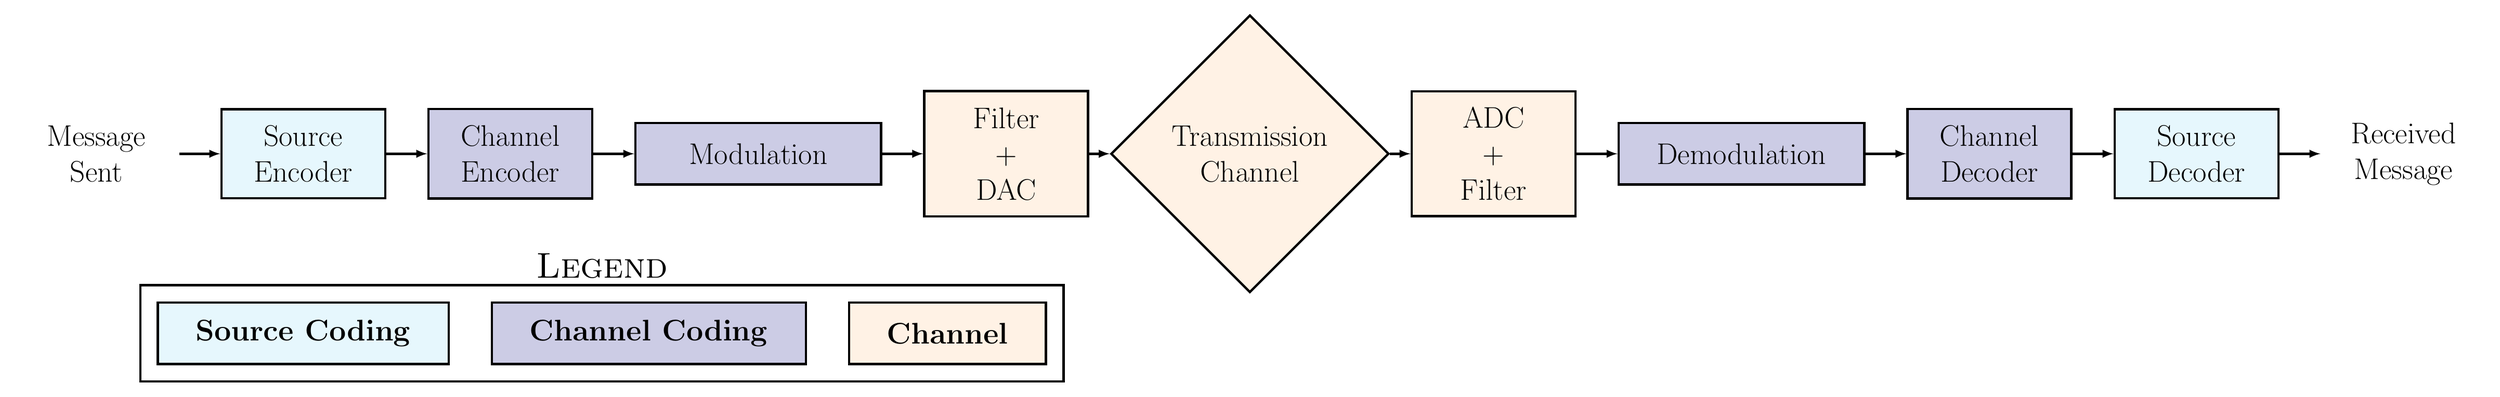
\begin{tikzpicture} [-latex,
    >=latex,
    auto,
    ultra thick,
    every node/.style={font=\huge},
    main node/.style={rectangle, draw, inner sep = 4mm,
        align=center}]

  \node [
    align=center,
    minimum height = 1.5cm,
    minimum width = 4cm,
  ] (m) at (0, 0) {Message\\Sent};

  \node [main node,
    fill=cyan!10,
    align=center,
    minimum height = 1.5cm,
    minimum width = 4cm,
    right = 1cm of m
  ] (srcenc) {Source\\Encoder};

  \node [main node,
    fill = NavyBlue!20,
    minimum height = 1.5cm,
    minimum width = 4cm,
    right = 1cm of srcenc
  ] (chanenc) {Channel\\Encoder};


  \node [main node,
    fill = NavyBlue!20,
    minimum height = 1.5cm,
    minimum width = 6cm,
    right = 1cm of chanenc
  ] (mod) {Modulation};

  \node [main node,
    fill = orange!10,
    minimum height = .75cm,
    minimum width = 4cm,
    right = 1 cm of mod
  ] (dac) {Filter\\$+$\\DAC};

  \node [main node,
    diamond,
    fill = orange!10,
    draw,
    align=center,
    %minimum height = 1.5cm,
    minimum width = 4cm,
    anchor = north,
    right = .5 cm of dac
  ] (chan)  {Transmission\\Channel};

  \node [main node,
    fill = orange!10,
    minimum height = .75cm,
    minimum width = 4cm,
    right = .5 cm of chan
  ] (adc) {ADC\\$+$\\Filter};

  \node [main node,
    % fill = red!60!gray!30!white,
    fill = NavyBlue!20,
    minimum height = 1.5cm,
    minimum width = 6cm,
    right = 1 cm of adc
  ] (demod)  {Demodulation};

  \node [main node,
    fill = NavyBlue!20,
    % fill = gray!40!white,
    minimum height = 1.5cm,
    minimum width = 4cm,
    right = 1 cm of demod
  ] (chandec) {Channel\\Decoder};

  \node [main node,
    fill=cyan!10,
    minimum height = 1.5cm,
    minimum width = 4cm,
    right = 1cm of chandec
  ] (srcdec) {Source\\Decoder};

  \node [
    align=center,
    minimum width = 4cm,
    right = 1cm of srcdec,
  ] (mp)  {Received\\Message};

  \node [main node,
    fill=cyan!10,
    minimum height = 1.5cm,
    minimum width = 4cm,
    below = 2.5 cm of srcenc,
  ] (legsrccod) {\phantom{O}\textbf{Source Coding}\phantom{O}};

  \node [main node,
    fill = NavyBlue!20,
    minimum height = 1.5cm,
    minimum width = 4cm,
    right = 1 cm of legsrccod,
  ] (legchncod) {\phantom{O}\textbf{Channel Coding}\phantom{O}};

  \node [main node,
    fill = orange!10,
    minimum height = 1.5cm,
    minimum width = 4cm,
    right = 1 cm of legchncod,
  ] (legchanel) {\phantom{O}\textbf{Channel}\phantom{O}};

  \node [main node,
    fill=none,
    fit = (legsrccod) (legchanel),
    inner sep = 4mm,
    label = \textsc{\Huge Legend},
  ] (legend) {};
  %%%%%%%%%%%%%%%%%%%%%%%%%%%%%%

  \draw (m.east) -> (srcenc.west);

  \draw (srcenc.east) -> (chanenc.west);

  \draw (chanenc.east) -> (mod.west);

  \draw (mod.east) -> (dac.west);

  \draw (dac.east) -> (chan.west);
  \draw (chan.east) -> (adc.west);

  \draw (adc.east) -> (demod.west);

  \draw (demod.east) -> (chandec.west);

  \draw (chandec.east) -> (srcdec.west);

  \draw (srcdec.east) -> (mp.west);
\end{tikzpicture}


\end{document}
